\section{Impedancia de entrada}

\subsection{Circuito inversor}

Partiendo del hecho que la impedancia de entrada puede expresarse como el cociente entre la tensión sobre la fuente de entrada y la corriente que circula a través suyo, y teniendo en cuenta las relaciones para el circuito inversor, se plantea que:

$$Z_{in}=\frac{V_{in}}{I_{1}}$$

$$v_{out}=-A_{v_{ol}}v^{-}$$

Observando las corrientes sobre la Figura \ref{fig:circInv}, se tiene que:

$$I_{1}R_{1}=V_{in}+\frac{V_{out}}{A_{v_{ol}}}=V_{in}+\frac{V_{in}H(s)}{A_{v_{ol}}}$$

Volviendo a la primera relación y simplificando, se obtiene lo siguiente:

$$Z_{in}=\frac{V_{in}}{I_{1}}=\frac{R_{1}}{1+\frac{H(s)}{A_{v_{ol}}}}$$

\begin{equation} \label{eq:zin1}
	Z_{in}(s)=\frac{R_{1}A_{ol}+R_{1}k+\frac{R_{1}A_{ol}}{w_{b'}}s}{s(\frac{1}{w_{b'}}+\frac{G_{id}}{w_{b}})+G_{id}+\frac{k}{A_{ol}}+1}
\end{equation}

En el caso que $A_{v_{ol}}\underset{\infty }{\rightarrow} Z_{in}=R_{1}$

Para medir la impedancia de entrada, en cada caso se agregó una resistencia similar al valor nominal de $R_{1}$ en serie, midiendo la tensión entre sus bornes y obteniendo la corriente que circula a través de ella. Para la simulación, se utilizaron los mismos circuitos que se mencionaron anteriormente. 

\begin{figure}[H]
	\centering
	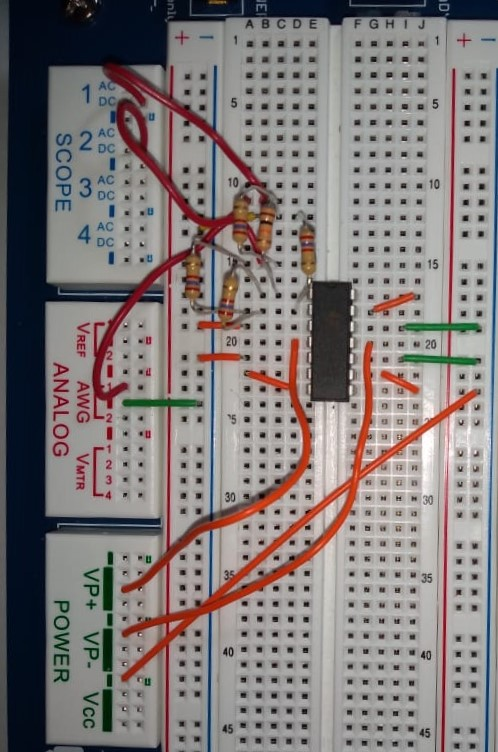
\includegraphics[scale=0.4]{./Imagenes/Inv2Zin.jpeg}
	\caption{Circuito inversor Caso 2 en el Digilent Electronics Explorer. Medición impedancia de entrada.}
	\label{fig:circInv}
\end{figure}

Graficando la expresión teórica ideal para la impedancia de entrada junto a los datos obtenidos de la simulación y de las mediciones, se obtuvieron los siguientes resultados:

\begin{figure}[H]
	\centering
		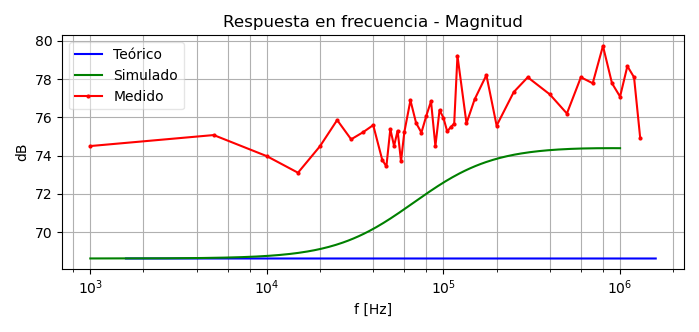
\includegraphics[width=.8\linewidth]{./Imagenes/InvCaso1ZinGain.png}  
		\caption{Inversor caso 1. Módulo de impedancia de entrada [dB]}
	\label{fig:circinvcaso1}
\end{figure}

\begin{figure}[H]
	\centering
		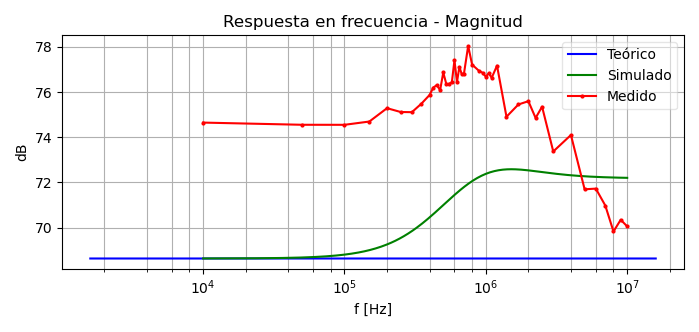
\includegraphics[width=.8\linewidth]{./Imagenes/InvCaso2ZinGain.png}  
		\caption{Inversor caso 2. Módulo de impedancia de entrada [dB]}
	\label{fig:circinvcaso1}
\end{figure}

\begin{figure}[H]
	\centering
		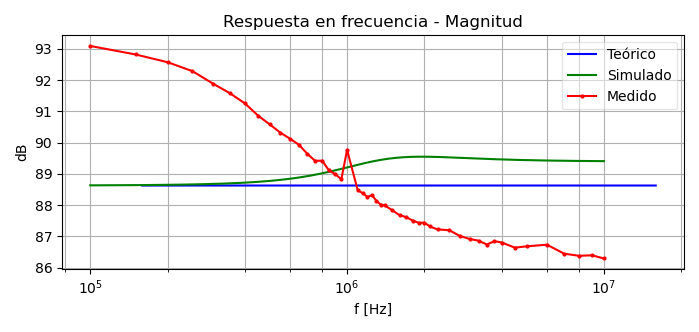
\includegraphics[width=.8\linewidth]{./Imagenes/InvCaso3ZinGain.png}  
		\caption{Inversor caso 3. Módulo de impedancia de entrada [dB]}
	\label{fig:circinvcaso1}
\end{figure}

En los tres casos se visualizan diferencias en el módulo de la impedancia de entrada. En los tres casos a bajas frecuencias la impedancia de entrada medida es bastante mayor que la teórica o la simulada. A bajas frecuencias los datos de la simulación coinciden con la expresión teórica ideal, tal como se esperaría y viene sucediendo en el análisis del circuito hasta ahora. En los casos 1 y 2 los datos medidos tienen un comportamiento similar a la simulación, a excepción del caso 3 en la que los datos medidos decaen constantemente con la frecuencia. 

\subsection{Circuito No Inversor}

Se parte de la relación entre tensión sobre la fuente de entrada y la corriente que circula por ella. 

$$Z_{in}=\frac{V_{in}}{I_{3}}$$

Considerando la relación de corrientes y resolviendo, se obtiene que:

$$v^{+}=V_{in}-I_{3}R_{3}$$

$$V^{-}=\frac{R_{1}}{R_{1}+R_{2}}V_{out}$$

$$V_{out}=H(s)V_{in}$$

$$Z_{in}(s)=\frac{-R_{3}(\frac{s}{\frac{w_{b}q_{2}}{q_{1}}}+1)A_{ol}}{A_{ol}\frac{(R_{1}+R_{2})R_{4}}{q_{2}}(\frac{s}{w_{b}}+1)-A_{ol}(\frac{s}{\frac{w_{b}q_{2}}{q_{1}}}+1)}$$

En el caso que $A_{v_{ol}}\underset{\infty }{\rightarrow} Z_{in}= R_{3}+R_{4}$

Se ocupará el modelo ideal para estudiar los resultados. 

Se midió de la misma forma antes descripta: una resistencia en serie con $R_{3}$ de magnitud similar a la impedancia de entrada ideal, obteniendo así la corriente y caída de tensión sobre esa resistencia y, con ello, el cálculo de la impedancia de entrada. Se superpuso el modelo teórico ideal con los datos de la simulación y los medidos, obteniendo los siguientes gráficos.

\begin{figure}[H]
	\centering
		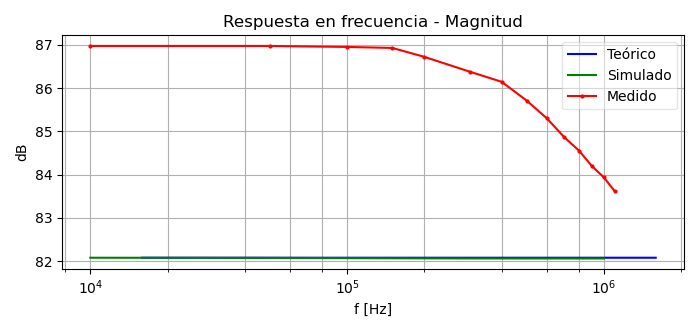
\includegraphics[width=.8\linewidth]{./Imagenes/NoInvCaso1ZinGain.png}  
		\caption{No inversor caso 1. Módulo de impedancia de entrada [dB]}
	\label{fig:circinvcaso1}
\end{figure}

\begin{figure}[H]
	\centering
		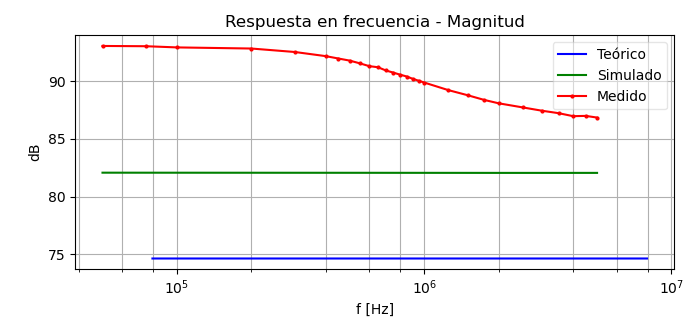
\includegraphics[width=.8\linewidth]{./Imagenes/NoInvCaso2ZinGain.png}  
		\caption{No inversor caso 2. Módulo de impedancia de entrada [dB]}
	\label{fig:circinvcaso1}
\end{figure}

\begin{figure}[H]
	\centering
		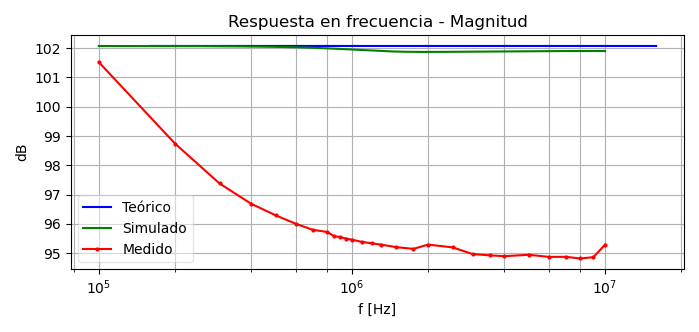
\includegraphics[width=.8\linewidth]{./Imagenes/NoInvCaso3ZinGain.png}  
		\caption{No inversor caso 3. Módulo de impedancia de entrada [dB]}
	\label{fig:circinvcaso1}
\end{figure}

Nuevamente, la magnitud de la impedancia de entrada medida es mayor a la simulada o a la teórica. En los datos de la simulación, se observa que la impedancia de entrada permanecería casi constante en respuesta a la frecuencia; sin embargo, en los datos medidos se observa una caída de la magnitud para frecuencias mas altas. 